\chapter{Гауссовская линейная модель} 

\begin{definition}
    Случайный вектор $ \xi = (\xi_1, \ldots, \xi_n)^T $ имеет \red{гауссовское (нормальное) распределение}, если его характеристическая функция имеет вид:
    $$\varphi_{\xi}(t)=Ee^{it^T\xi} = e^{it^Ta - \frac{1}{2}t^TKt}$$
    \noindentгде $ t = (t_1, \ldots, t_n)^T \in \mathbb{R}^n, \; a = (a_1, \ldots, a_n)^T, \; K = (k_{ij}) $ с $ i,j = 1, \ldots, n, \; k_{ij} \in \mathbb{R}, \; K = K^T, \; K \geqslant 0, \; i^2 = -1$. \\Обозначение: $ \xi \sim N(a,K) $.
 \end{definition}

\section{Свойства Гауссовского закона}

\begin{itemize} 
  \item[$1)$] 
    $ \xi_j \sim N(a_j, k_{jj}) $
    \begin{Proof}
    	Действительно, $\displaystyle \varphi_{\xi_j}(t_j) = \varphi(0, \ldots, t_j, 0, \ldots, 0) = e^{it_ja_j-\frac{1}{2}t_j^2k_{jj}} $, а это -- характеристическая функция $ N(a_j, k_{jj}) $ 
    \end{Proof}
  \item[$2)$]
    $ k_{ij} = Cov(\xi_i, \xi_j)$, $ k_{ii} = D\xi_i $, $ K $ -- \blue{ковариационная матрица} $ \xi $.
    \begin{Proof}
      Из свойства $1)$ следует, что $ a = E\xi $ и, если $ \tilde{\xi} = \xi - a $, то $ E\tilde{\xi} = 0 $. $ \displaystyle \varphi_{\tilde{\xi}}(t) = e^{-it^Ta}\varphi_{\xi}(t) = e^{-\frac{1}{2}t^TKt} $. Отсюда имеем:
      $$ \displaystyle E\tilde{\xi_i}\tilde{\xi_j} = Cov(\xi_i, \xi_j) = - \dfrac{\partial^2\varphi_{\tilde{\xi}}(0)}{\partial t_i\partial t_j} = k_{ij} $$
    \end{Proof}
  \item[$3)$] 
    Если $ \xi \sim N(a,K) $, то $ \lbrace \xi_1, \ldots, \xi_n \rbrace $ независимы тогда и только тогда, когда $ K $ -- диагональная матрица.
    \begin{Proof}
      $ K $ -- диагональная тогда и только тогда, когда: 
      $$ \varphi_{\xi}(t) = e^{it^Ta - \frac{1}{2} \sum\limits_{t = 1}^n k_{ii}t_i^2} = \prod\limits_{i = 1}^n e^{it_ia_i - \frac{1}{2}k_{ii}t_i^2} = \prod\limits_{i = 1}^n \varphi_{\xi_i}(t)$$ 
      Это есть необходимое и достаточное условие независимости.
    \end{Proof}
    \begin{conseq}
      Если $ \eta \sim N(0, E_n) $, то $ \lbrace \eta_1, \ldots, \eta_n \rbrace $ -- н.о.р. $ N(0, 1)$ сл.в.
    \end{conseq}
  \item[$4)$] 
    Если $ \xi \sim N(a, K) $, а $ \eta = A\xi + b $, где $ A $ -- матрица размера $ (m\times n) $, $ b = (b_1, \ldots, b_m)^T \in \mathbb{R}^m$, то $ \eta \sim N(Aa + b, AKA^T) $
    \begin{Proof}
      $$ \begin{gathered} 
        \varphi_{\eta}(s)=Ee^{is^T(A\xi + b)}=e^{is^Tb}Ee^{i(A^Ts)^T\xi} = e^{is^Tb}e^{i(A^Ts)^Ta - \frac{1}{2}(A^Ts)^TK(A^Ts)}= \\ 
        = e^{is^T(Aa + b) - \frac{1}{2}s^T(AKA^T)s}\text{ -- х.ф., соответствующая сл.в.} \sim  N(Aa + b, AKA^T) \end{gathered}$$.
    \end{Proof}

    Пусть $C$ такая ортогональная матрица $(CC^T = E_n$, т.е. стр. орт.$)$, что $ CKC^T = D$, где $\displaystyle D = 
    \begin{pmatrix}
      d_1 & 0 & \ldots & 0\\
      0 & d_2 & \ldots & 0\\
      \vdots & \vdots & \ddots & \vdots\\
      0 & 0 & \ldots & d_n
    \end{pmatrix}$, $ d_i \geqslant 0$ -- собственные числа $ K $.
    
    Тогда $ K = C^TDC $. Положим $\displaystyle D^{\frac{1}{2}} := 
    \begin{pmatrix}
    \sqrt{d_1} & 0 & \ldots & 0\\
    0 & \sqrt{d_2} & \ldots & 0\\
    \vdots & \vdots & \ddots & \vdots\\
    0 & 0 & \ldots & \sqrt{d_n}\\
    \end{pmatrix}, \; K^{\frac{1}{2}} := C^TD^{\frac{1}{2}}C$.
    
    Тогда имеем следующие свойства:
    \begin{itemize}
      \item[$\bullet$] 
        $ K^{\frac{1}{2}} = (K^{\frac{1}{2}})^T $;
      \item[$\bullet$] 
        $ K^{\frac{1}{2}}K^{\frac{1}{2}} = K $;
      \item[$\bullet$] 
        Если $ K > 0 $, то $ K^{\frac{1}{2}}KK^{-\frac{1}{2}} = E_n $;
      \item[$\bullet$] 
        $ det(K^{\frac{1}{2}}) = (detK)^{\frac{1}{2}} $
    \end{itemize}
  
  \item[$5)$] 
    Если $ \xi \sim N(a, K) $ и $ K > 0 $, то существует плотность вероятности по мере Лебега $ \displaystyle p_{\xi}(x) = \dfrac{1}{(2 \pi)^{\frac{n}{2}} det(K^{\frac{1}{2}}) }e^{-\frac{1}{2}(x - a)^TK^{-1}(x - a)} $.
    \begin{Proof}
      Положим $ \eta := K^{-\frac{1}{2}}(\xi - a) $. Тогда $ E\eta = K^{-\frac{1}{2}}E(\xi - a) = 0 $, $ E\eta\eta^T = K^{-\frac{1}{2}}E(\xi - a)(\xi - a)^T K^{-\frac{1}{2}} = K^{-\frac{1}{2}}KK^{-\frac{1}{2}} = E_n$.
      
      В силу свойства $2)$ имеем $ \eta_n \sim N(0, E_n) $, а также:
      $$ \xi = K^{\frac{1}{2}}\eta + a \eqno(1)$$
      
      \begin{problem}
        Если $ Z $ и $ Y $ -- случайные векторы размерности n, $ A $ -- матрица $ (n\times n) $ такая, что $ det(A) \neq 0 $, $ Z = AY + a $, то: 
        $$ p_z = \dfrac{1}{det(A)}p_y(A^{-1}(x - a)) \eqno(2)$$
      \end{problem}
      Если $ \eta \sim N(0, E_n) $, то $$\begin{gathered} p_{\eta}(x) = \prod\limits_{i = 1}^np_{\eta_i}(x_i) = \dfrac{1}{(2 \pi)^\frac{1}{2}}e^{-\frac{1}{2}\sum\limits_{i = 1}^nx_i^2} = \dfrac{1}{(2 \pi)^{\frac{n}{2}}}e^{-\frac{1}{2}x^Tx}  \end{gathered}$$. В силу (1), (2) имеем $$ \begin{gathered} p_{\xi}(x) = \dfrac{1}{(2 \pi)^{\frac{n}{2}} det(K^{\frac{1}{2}})}p_{\eta}(K^{-\frac{1}{2}}(x-a)) = \dfrac{1}{(2 \pi)^{\frac{n}{2}}(detK)^{\frac{1}{2}}}e^{-\frac{1}{2}(x-a)^TK^{-1}(x-a)} \end{gathered}$$.
    \end{Proof}
\end{itemize}

\begin{remem}
  Из раздела 4. Если $ \lbrace \xi_1, \ldots, \xi_k \rbrace $ -- н.о.р. $ N(0, 1) $ сл.в., то $ \eta_k = \xi_1^2 + \ldots + \xi_k^2 $ имеет распределение \textit{$ \chi^2 $ Пирсона (хи-квадрат Пирсона) с $ k $ степенями свободы}: $ \eta_k \sim  \chi^2(k)$. Тогда $ E\eta_k = k, \; D\eta_k = 2k$.
\end{remem}

\begin{lemma}
  Пусть $ \xi \sim N(0, \sigma^2E_n), \sigma^2 > 0 $. Тогда:
  \begin{itemize}
    \item[$1)$] 
      если $ C $ -- ортогональная матрица размера $ n \times n $, а $ \eta = C\xi $, то: 
      $$ \eta \sim N(0, \sigma^2E_n), \text{ т.е. } \xi \stackrel{d}{=} \eta $$
    \item[$2)$] 
      если $ h_1, \; h_2 $ -- линейные подпространства $ \mathbb{R}^n $, $ h_1 \bot h_2 $, то $ \{proj_{h_i}\xi\}, \; i = 1, 2 $ являются независимыми гауссовскими векторами: 
      $$ E \; proj_{h_i}\xi = 0, \; \dfrac{1}{\sigma^2} |proj_{h_i}\xi|^2 \sim \chi^2(dim\;h_i) $$
  \end{itemize}
\end{lemma}
\begin{Proof}
  Докажем по пунктам.
  \begin{itemize}
    \item[$1)$] 
      $ E\eta = EC\xi = CE\xi = 0, \; E\eta\eta^T = C(\sigma^2E_n)C^T = \sigma^2E_n $. Значит, $ \eta \sim N(0, \sigma^2E_n) $ по свойству 4.
    \item[$2)$] 
      Выберем в $ \mathbb{R}^n $ ортонормированный базис $\underbrace{e_1, \ldots, e_p, }_{\text{базис }  h_1 }\underbrace{ e_{p + 1}, \ldots, e_{p + m}, }_{\text{базис } h_2 }$ $ \ldots, e_n $. Тогда $ dim(h_1) = p $. Имеем: 

      $$proj_{h_1}\xi = \sum\limits_{i = 1}^p\underbrace{ (\xi^Te_i) }_{ = \eta_i }e_i = \sum\limits_{i = 1}^p\eta_ie_i \eqno(3)$$
    \begin{center}
      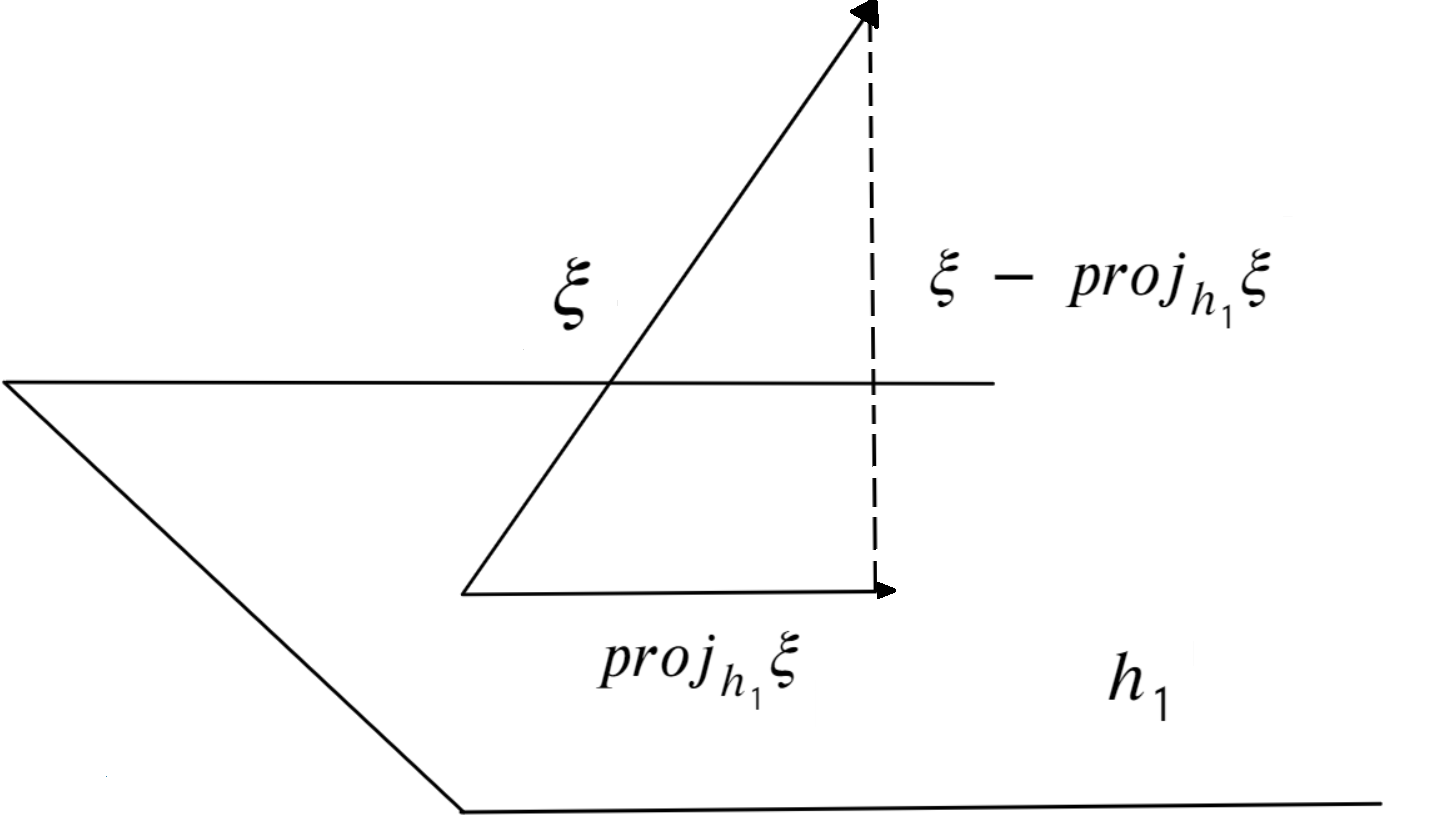
\includegraphics[scale=0.3]{lec7im1}
    \end{center}
  \end{itemize}

  Действительно, $ \displaystyle proj_{h_1}\xi = \sum\limits_{i = 1}^pb_ie_i$. Также $\displaystyle (\xi - proj_{h_1}\xi^Te_j = 0)$ для $ j = 1, \ldots, p $, $ \xi^Te_j = b_j = \eta_j$, тогда $(3)$ верно. Аналогично получаем:
  $$proj_{h_2}\xi = \sum\limits_{i = p + 1}^{p + m}\eta_ie_i \eqno(4)$$ 

  Если $ \eta = (\eta_1, \ldots, \eta_n)^T = (e_1^T, \ldots, e_n^T)^T\xi $, то $ (e_1^T, \ldots, e_n^T)^T $ -- ортонормированная матрица. В силу пункта $1)$ этой леммы $ \eta \sim N(0, \sigma^2E_n) $. По $(3)$, $(4)$ $ proj_{h_1}\xi $ и $ proj_{h_2}\xi $ независимы, так как определяются $ \eta_1, \ldots, \eta_p $ и $ \eta_{p + 1}, \ldots, \eta_{p + m} $ соответственно.

  Очевидно, что $ \lbrace proj_{h_i}\xi \rbrace, \; i = 1, 2$ -- гауссовские векторы, т.е. получаются линейным преобразованием гауссовского вектора $ \eta $. Например: 
  $$ proj_{h_1}\xi =  \underbrace{(e_1, \ldots, e_p)}_{\text{матрица }(n \times p )}(\eta_1, \ldots, \eta_p)^T$$ 
  Так же очевидно, что $ E \; proj_{h_1}\xi = 0 $, т.к. $ E\eta = 0 $. Наконец:
  $$\dfrac{1}{\sigma^2}|proj_{h_1}\xi|^2 = \dfrac{1}{\sigma^2} \left| \sum\limits_{i = 1}^p \eta_ie_i\right|^2 = \dfrac{1}{\sigma^2} \sum\limits_{i = 1}^p\eta_i^2 = \sum\limits_{i = 1}^p \left(\dfrac{\eta_i}{\sigma}\right)^2 \sim \chi^2(p = dim\left(h_1)\right)$$
\end{Proof}










\section{Линейная Гауссовская модель.}

$ X \sim N(l, \sigma^2E_n), \; \sigma^2 > 0, \sigma^2 $ -- неизвестно, $ l \in h $ -- неизвестно. $ h $ -- известное линейное подпространство $ \mathbb{R}^n, \; dimh = p < n. $ Если $ \varepsilon := x - l  $, то: 
$$X = l + \varepsilon, \; \varepsilon \sim N(0, \sigma^2E_n), l \in h\eqno(5)$$ 
Неизвестный параметр $ \theta \in \mathbb{R}^{n + 1}, \theta^T = (l^T, \sigma
^2)$. Пусть $ h^{\bot} $ -- ортогональное дополнение к $ h $ в $ \mathbb{R}^n $, то есть множество векторов из $ \mathbb{R}^n,  $ перпендикулярных $ h $. Тогда $ dim(h^{\bot}) = n - p $, и имеем:
$$ \forall x \in \mathbb{R}^n \; x = proj_hx + proj_{h^{\bot}} \eqno(6)$$

Найдем достаточную статистику для $ \theta $. Плотность $ X $ засчет $(5)$, $(6)$ есть 
$$ \begin{gathered}
  p(x, l, \sigma^2) = (\dfrac{1}{\sqrt{2 \pi}\sigma})^ne^{-\frac{1}{2\sigma^2}|x-l|^2}  \stackrel{\text{в силу} (6)}{=} (\dfrac{1}{\sqrt{2 \pi}\sigma})^n e^{-\frac{1}{2\sigma^2}|(proj_hx - l) + proj_{h^{\bot}}|^2} = \\
  = (\dfrac{1}{\sqrt{2 \pi}\sigma})^n e^{-\frac{1}{2\sigma^2}(|proj_hx - l|^2 + |proj_{h^{\bot}}|^2)} = \psi(T(x), \theta)h(x)
\end{gathered}$$ 
где $ T(x) = \left((proj_hx)^T, |proj_{h^{\bot}}|^2 \right)^T, h(x) = 1 $. В силу критерия факторизации $ T(x) $ -- достаточная статистика. Примем без доказательства, что это -- полная статистика.
 
\begin{itemize}
  \item[$1)$] 
    \colorbox{DarkSeaGreen}{Оптимальная оценка $ l $.} $ proj_hX = proj_hl = proj_h\varepsilon$, тогда $E\;proj_hX = l + E\;proj_h\varepsilon = l $ в силу пункта $2)$ леммы \ref{cha:7/lemma:1}. Итак, $ proj_hX $ есть функция полной достаточной статистики $ Eproj_hX = l $. По лемме \ref{cha:7/lemma:2} Лемана-Шеффе $ \hat{l^n} := proj_hX $ -- оптимальная оценка $ l $.
  \item[$2)$] 
    \colorbox{DarkSeaGreen}{Оптимаьная оценка $ \sigma^2 $}. $ proj_{h^{\bot}}X = proj_{h^{\bot}}l + proj_{h^{\bot}}\varepsilon = proj_{h^{\bot}}\varepsilon $. 

    В силу пункта $2)$ леммы \ref{cha:7/lemma:1} имеем:
    $$\dfrac{1}{\sigma^2}|proj_{h^{\bot}}X|^2 = \dfrac{1}{\sigma^2}|proj_{h^{\bot}}\varepsilon|^2 \sim \chi^2(n-p)\eqno(7)$$ 
    Значит, $ E\dfrac{1}{\sigma^2}|proj_{h^{\bot}}\varepsilon|^2 = n - p, \; E\dfrac{1}{n - p}|proj_{h^{\bot}}X|^2 = \sigma^2$. В силу леммы \ref{cha:7/lemma:2} Лемана-Шеффе $ \hat{s_n}^2 := \dfrac{1}{n - p}|proj_{h^{\bot}}X|^2 $ -- оптимальная оценка $ \sigma^2. $ Кроме того, по $(7)$ имеем:
    $$ \dfrac{(n - p)\hat{s_n}^2}{\sigma^2} = \dfrac{1}{\sigma^2}|proj_{h^{\bot}}X|^2 \sim \chi^2(n - p) \eqno(8)$$
  \item[$3)$] 
    \colorbox{DarkSeaGreen}{Независимость $ \hat{l_n} $ и $ \hat{s_n}^2 $}. В силу пункта $2)$ леммы \ref{cha:7/lemma:1} $ proj_hX = l + proj_h\varepsilon $ и $ proj_{h^{\bot}} X = proj_{h^{\bot}}\varepsilon  $ независимы, значит $\hat{l_n} \text{ и } \hat{s_n}^2 $ независимы.
\end{itemize}

В силу леммы \ref{cha:7/lemma:2} Лемана-Шеффе $ (\hat{l_n}^T, \hat{s_n}^2)^T $ -- оптимальная оценка вектора $ \theta = (l^T, \sigma^2)^T$. 
$$ \hat{l_n} = proj_hX = \underset{Y \in h}{argmin}|X-Y| = \underset{Y \in h}{argmin}|X-Y|^2 = \underset{Y \in h}{argmin}\sum\limits_{i = 1}^n(X_i - Y_i)^2$$
Поэтому $ \hat{l_n} $ и $ \hat{s_n}^2 = \dfrac{1}{n - p}|X - proj_hX|^2 $ называются \red{оценками по методу наименьших квадратов}. 
\begin{center}
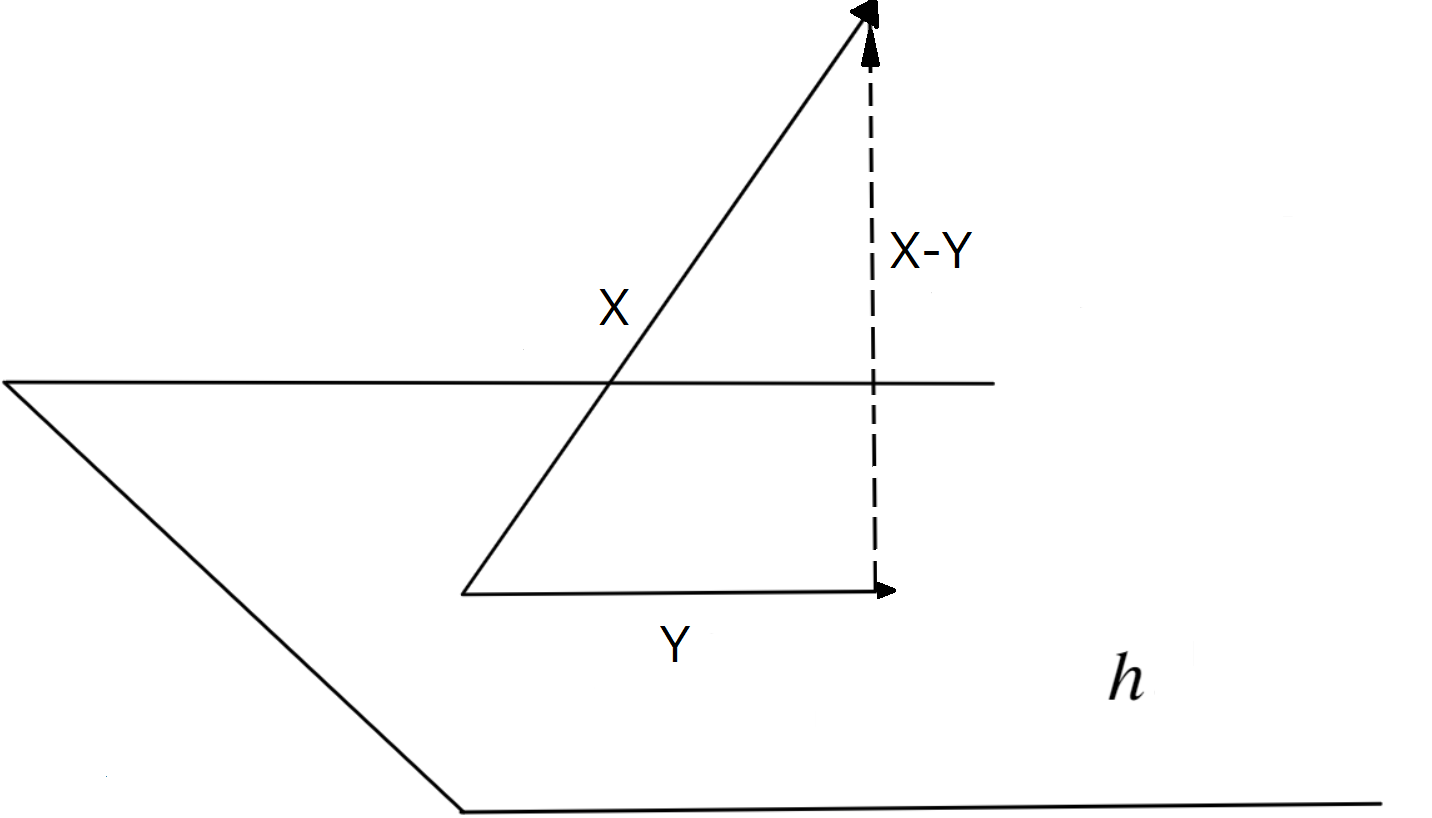
\includegraphics[scale=0.3]{lec7im2}
\end{center}

Выберем в $ h $ базис, пусть столбцы матрицы размера $ (n \times p)$  $Z = \{z_{ij}\}$, $i = 1, \dots, n, j = 1, \ldots, p $ будут базисными векторами. Тогда для некоторого $ c = (c_1, \ldots, c_p)^T $ имеем $ l = Zc $, и линейная модель (5) получает вид:
$$ X = Zc + \varepsilon\eqno(9)$$ 

Если $ z_i^T $ -- строки матрицы $ Z $, то (9) эквивалентно:
$$ X_i = z_i^Tc + \varepsilon_i, \; i = 1, \ldots, n \eqno(10)$$ 

Соотношения (9) и (10) задают \red{гауссовскую линейную регрессию}, это -- еще одна форма записи линейной модели (5).

В (9) неизвестный параметр $ \theta, \; \theta^T = (c^T, \sigma^2), dim(\theta) = p + 1 $. Матрица $ Z $ -- \red{регрессионная матрица}, она известна. $ X $ -- наблюдение. \textit{Надо оценить $ \theta, $} то есть $ \sigma^2. $

\begin{definition}
\red{Оценкой наименьших квадратов (н.к.) $ \hat{c_n} $ вектора $ c $} называется решение задачи $ |X - Z\alpha|^2 = \sum\limits_{i = 1}^n(X_i - z_i^T\alpha)^2 \longrightarrow \underset{\alpha \in \mathbb{R}^p}{min} $, то есть $ \hat{c_n} = \underset{\alpha \in \mathbb{R}^p}{argmin}|X-Z\alpha|$. 
\end{definition}

Пусть $ h $ -- линейное пространство столбцов Z, то есть столбцы Z -- базисные векторы h. Ясно, что $ |X - Z\alpha|^2 $ достигает минимума при $ \alpha = \hat{c_n} $ таком, что $ X-Z\hat{c_n} \bot h $, то есть $ Z^T(X - Z\hat{c_n}) = 0, \; Z^TX = Z^TZ\hat{c_n}$, тогда получаем:
$$\hat{c_n} = (Z^TZ)^{-1}Z^TX \eqno(11)$$
\begin{center}
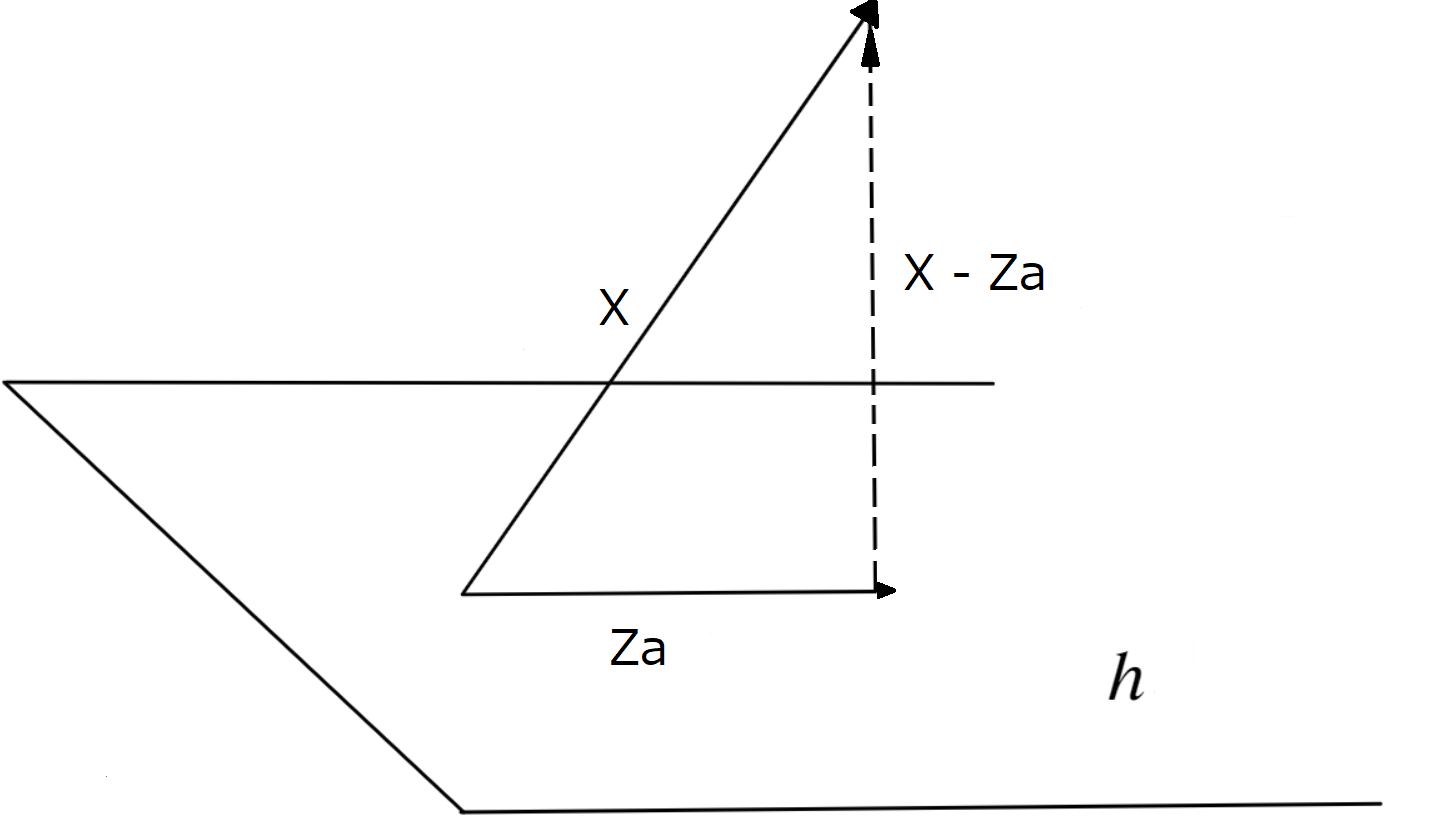
\includegraphics[scale=0.3]{lec7im3}
\end{center}

\textit{Отметим еще раз: $ Z\hat{c_n} = proj_hX $}. Матрица $ Z^TZ $ в (11) невырождена, так как при $ \alpha \neq 0 \; \alpha^TZ^TZ\alpha = |Z\alpha|^2 > 0$ из-за независимости столбцов Z.

\colorbox{DarkSeaGreen}{Оценка н.к. для $ \sigma^2 $}: $ \hat{s_n}^2 = \dfrac{1}{n - p}|X-Z\hat{c_n}|^2 $. Разумеется: 
$$ \displaystyle \hat{s_n}^2 = \dfrac{1}{n - p}\sum\limits_{i = 1}^n(x_i - z_i^T\hat{c_n})^2, \; \hat{s_n}^2 = \dfrac{1}{n-p}|proj_{h^{\bot}}X|^2 $$

\begin{definition}
  Вектор $ X - Z\hat{c_n} = (\hat{\varepsilon_1}, \ldots, \hat{\varepsilon_n})^T $  называют \red{вектором остатков}, а $ \hat{s_n}^2 $ -- \red{остаточной дисперсией.}
\end{definition}

\begin{theorem}\label{cha:8/the:1}
  Имеем несколько утверждений:
  \begin{itemize}
    \item[$1)$] 
      $ \hat{c_n}  \sim N(c, \sigma^2(Z^TZ)^{-1}), \; \dfrac{(n - p)\hat{s_n}^2}{\sigma^2} \sim \chi^2(n - p), \; E_{c, \sigma^2}\hat{s_n}^2 = \sigma^2, \; D_{c, \sigma^2}\hat{s_n}^2 = \dfrac{2\sigma^4}{n - p} $.
    \item[$2)$] 
      $ \hat{c_n} $ и $ \hat{s_n}^2 $ независимы. 
    \item[$3)$] 
      Оценки $ \hat{c_n} $ и $ \hat{s_n}^2 $ -- оптимальные оценки $ c $ и $ \sigma^2 $ соответственно.
  \end{itemize}
\end{theorem}
\begin{Proof}
  \begin{itemize}
    \item[$1)$] 
      \colorbox{DarkSeaGreen}{Распределение $ \hat{c_n} $}. В силу (11) $ \hat{c_n} $ есть линейное преобразование гауссовского вектора Х. В силу свойства 4 для гауссовких векторов, $ \hat{c_n} $ -- гауссовский вектор. 
      $$ E_{c, \sigma^2}\hat{c_n} = E_{c, \sigma^2}(Z^TZ)^{-1}Z^TX = (Z^TZ)^{-1}Z^TE_{c, \sigma^2}X = (Z^TZ)^{-1}Z^TZc = c $$
      То есть $ \hat{c_n} $ -- несмещенная оценка. 
      $$\begin{gathered}
        D_{c, \sigma^2}\hat{c_n} = E_{c, \sigma^2}(\hat{c_n} - c)(\hat{c_n} - c)^T = E_{c, \sigma^2}(Z^TZ)^{-1}Z^T(\varepsilon\varepsilon^T)Z(Z^TZ)^{-1} = \\
        = (Z^TZ)^{-1}Z^T(\sigma^2E_n)Z(Z^TZ)^{-1} = \sigma^2 (Z^TZ)^{-1}
      \end{gathered}$$
      Итак, $ \hat{c_n} \sim N(0, \sigma^2(Z^TZ)^{-1}) $.

      \colorbox{DarkSeaGreen}{Распределение $ \hat{s_n}^2 $}. Модель (9) эквивалентна $ X = l + \varepsilon $, где $ l = Zc, \; l \in h, \; h  \text{ -- пространство столбцов Z} $. В силу (13) и (8) $ \dfrac{(n-p)\hat{s_n}^2}{\sigma^2} \sim \chi^2(n - p ) $. Значит, $ E_{c, \sigma^2}\hat{s_n}^2 = \dfrac{\sigma^2}{n - p}\eta_{n - p} = \sigma^2 $. То есть $ \hat{s_n}^2 $ -- несмещенная оценка $ \sigma^2. $
    \item[$2)$] 
      В силу $(12)$ имеем:
      $$\hat{c_n} = (Z^TZ)^{-1}Z^TZ\hat{c_n} = (Z^TZ)^{-1}Z^Tproj_hX \eqno(14)$$
      Т.к. $proj_hX $ и $ proj_{h^{\bot}}X $ независимы, то $ \hat{c_n} $ и $ \hat{s_n}^2 $ независимы.
    \item[$3)$] 
      Докажем оптимальность $ \hat{c_n} $, оптимальность $ \hat{s_n}^2 $ доказывается аналогично. 

      Уже имеем, что $ \hat{c_n} $ -- несмещенная. Надо доказать, что: 
      $$ D_{c, \sigma^2}\hat{c_n} = D_{l, \sigma^2} \widehat{c_n} \; \forall l, \; \sigma^2 > 0\eqno(15)$$ 
      где $ \widehat{c_n} $ -- любая несмещенная оценка с. 

      У нас $ l = Zc, $ то есть $ Z^Tl = Z^TZc, \; c = (Z^TZ)^{-1}Z^Tl $. Имеем взаимно однознаное отображение $ c \longleftrightarrow l, \; l \in h, \; c \in \mathbb{R}^p $. Иогда левая часть (15) в силу (14) равна $ \displaystyle D_{c, \sigma^2}(Z^TZ)^{-1}Z^Tproj_hX $ -- ковариация функции полной достаточной статистики $ \left((proj_hx)^T, |proj_{h^{\bot}}|^2\right)^T $ для параметра $ (l^T, \sigma^2)^T $. Правая часть (15) есть $ E_{l, \sigma^2}\widehat{c_n} $. В силу леммы \ref{cha:7/lemma:2} Лемана-Шеффе $ \displaystyle D_{l, \sigma^2}(Z^TZ)^{-1}Zproj_hX \leq  D_{l, \sigma^2}\widehat{c_n} \; \forall l \in h, \; \sigma^2.$ Значит, (15) -- верно.
  \end{itemize}
\end{Proof}


\section{Пример(Гауссовская выборка.)}

\begin{example}
  Пусть $ X = (X_1, \ldots, X_n)^T $, где $ \lbrace X_i \rbrace $ -- н.о.р., $ X_1 \sim N(a, \sigma^2) $. Построим оптимальные оценки $ a $ и $ \sigma^2 $, исследуем их свойства.

  Пусть $ \varepsilon_i = X_i - a, \; i = 1, \ldots, n. $ Тогда:
  $$ X_i = a + \varepsilon_i, \; i = 1, \ldots, n; \; \lbrace \varepsilon_i \rbrace \text{ -- н.о.р., } \varepsilon_1 \sim N(0, \sigma^2) \eqno(16)$$

  Уравнение (16) -- частный случай линейной регрессии (10), где $ z_i^T = 1, \; c = a, \; p = 1. $ Значит, оптимальная оценка для $ a $ -- о.н.к., которая получается решением задачи $ \sum\limits_{i = 1}^n(X_i - \alpha)^2 \longrightarrow \underset{\alpha}{min} $. Эта задача эквивалентна решениюуравнения $ -2\sum\limits_{i = 1}^n(X_i - \alpha) = 0,$ корень -- $ \hat{\alpha_n} = \bar{X} $. 

  Оптимальная оценка для $ \sigma^2 $ -- остаточная дисперсия: $ \hat{s_n}^2 = \dfrac{1}{n - 1}\sum\limits_{i = 1}^n(X_i - \bar{X})^2 = S^2.$ Матрица $ Z = (z_1^T, \ldots, z_n^T)^T = (1, \ldots, 1)$, линейное пространство столбцов матрицы Z -- линейное пространство, натянутое на вектор $ (1, \ldots, 1)^T, \; l = (a_1, \ldots, a_n)^T $, оптимальная оценка $ l $ -- $ \hat{l} = Z\hat{c_n} = (\bar{X}, \ldots, \bar{X})^T $. Из теоремы \ref{cha:8/the:1} $ \bar{X} \sim N(a, \dfrac{\sigma^2}{n}), \; \dfrac{(n - 1)S^2}{\sigma^2} \sim \chi^2(n - 1). $

  $ \bar{X} $ и $ S^2 $ независимы. $ D_{a, \sigma^2}S^2 = \dfrac{2\sigma^2}{n - 1}. $ Ковариационная матрица вектора $ \hat{\theta_n} = (\bar{X}, S^2)^T $ есть $\displaystyle D_{a, \sigma^2}\hat{\theta_n} = 
  \begin{pmatrix}
    \dfrac{\sigma^2}{n}& 0\\
    0 & \dfrac{2\sigma^2}{n - 1}
  \end{pmatrix}$. Напомним, \red{матрица информации Фишера} (смотри раздел 5) равна $\displaystyle I(\theta) = 
  \begin{pmatrix}
    \dfrac{n}{\sigma^2}& 0\\
    0 & \dfrac{n}{2\sigma^2}
  \end{pmatrix}$, поэтому:
  $$D_{a, \sigma^2}\hat{\theta_n} = 
  \begin{pmatrix}
    \dfrac{\sigma^2}{n}& 0\\
    0 & \dfrac{2\sigma^2}{n - 1}
  \end{pmatrix} > I^{-1}(\theta) = 
  \begin{pmatrix}
    \dfrac{\sigma^2}{n}& 0\\
    0 & \dfrac{2\sigma^2}{n}
  \end{pmatrix}$$

  \textit{Значит, оценка $ (\bar{X}, S^2)^T $ является оптимальной оценкой $ (a, \sigma^2)^T $, но не является эффективной в $ C_{\mathbb{R}} $.}
\end{example}

\vspace{2cm}
\begin{definition}\label{cha:8/def:1}
  Пусть $ \xi_0, \ldots, \xi_k $ -- н.о.р. $ N(0, 1) $ сл.в. Случайная величина 
  $$\displaystyle t_k = \dfrac{\xi_0}{\sqrt{\dfrac{1}{k}(\xi_1^1 + \ldots + \xi_k^2)}} $$ 
  имеет \red{распределение Стьюдента с k степенями свободы}.
\end{definition}
То есть $ t_k = \dfrac{\xi_0}{\sqrt{\dfrac{1}{k}\eta_k}} $, где $ \xi_0 \sim N(0, 1), \; \eta_k \sim \chi^2(k), \; \xi_0 \text{ и } \eta_k $ независимы.\\

Поскольку $\displaystyle \dfrac{n^{\frac{1}{2}}(\bar{X - a})}{\sigma} \sim N(0, 1), \text{ а } \dfrac{(n - 1)S^2}{\sigma^2} \sim \chi^2(n - 1),  $ то: 
$$\displaystyle \dfrac{n^{\frac{1}{2}}(\bar{X - a})}{\sigma}\sqrt{\dfrac{1}{n-1}\dfrac{(n - 1)S^2}{\sigma^2}} = \dfrac{n^{\frac{1}{2}}(\bar{X} - a)}{S} \sim S(n - 1)$$

Величина $ \dfrac{n^{\frac{1}{2}}(\bar{X} - a)}{S} $ называется \red{стьюдентовой дробью}.












